% Asset ID: FA22FurtherKinematicsTikZ-001
% Source: Transcript notation recap
% Related lesson section: Core Theory; Visual Asset Integration
% Used placeholder:
% [VISUAL PLACEHOLDER: FA22FurtherKinematicsTikZ-001 | Source: Transcript notation recap | Insert from tikz/FA22FurtherKinematicsTikZ-001.tex | Purpose: Give a precise typeset diagram of the \(x\), \(v\), \(a\) ladder.]
% Purpose:
% Give a precise typeset diagram of the x, v, a ladder:
% differentiate down with respect to t, integrate up with respect to t.

\documentclass[tikz,border=8pt]{standalone}

\usepackage{amsmath}
\usepackage{amssymb}
\usetikzlibrary{arrows.meta, positioning, calc}

\definecolor{Canvas}{HTML}{FAF9F6}
\definecolor{Panel}{HTML}{FFFFF0}
\definecolor{Line}{HTML}{E5E5EA}
\definecolor{Text}{HTML}{2C2C2E}
\definecolor{Gold}{HTML}{C5A059}
\definecolor{Rose}{HTML}{FBEFEF}

\begin{document}

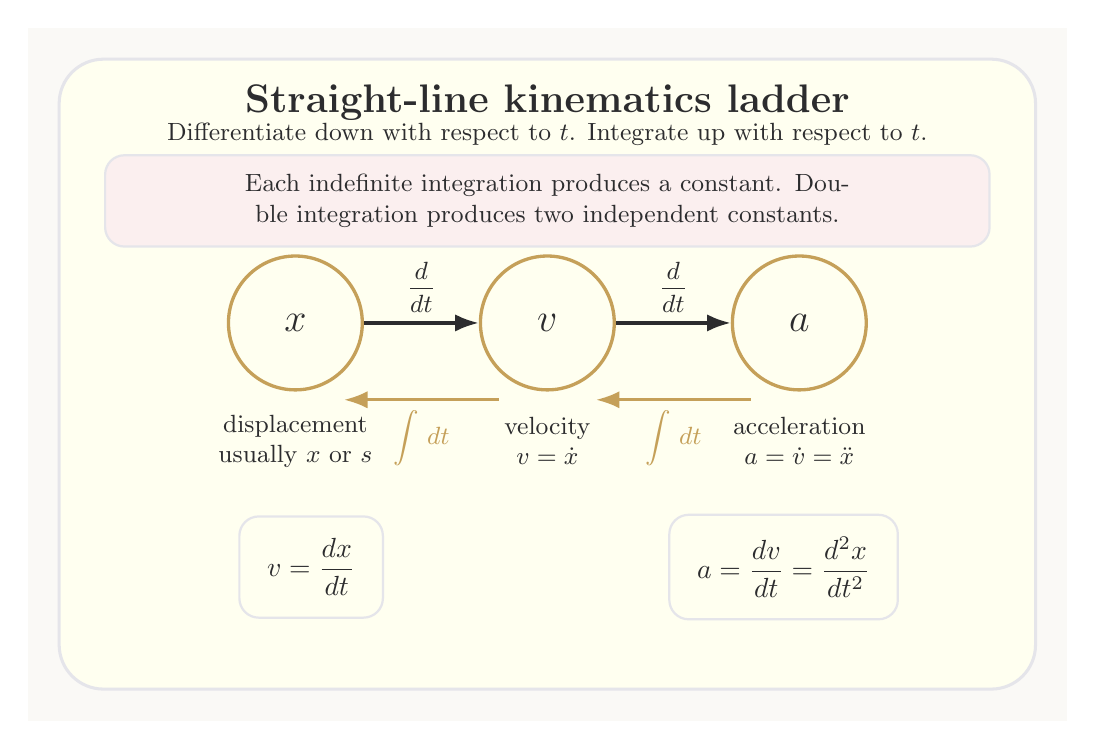
\begin{tikzpicture}[
  font=\sffamily,
  node distance=2.7cm,
  quantity/.style={
    circle,
    draw=Gold,
    line width=1.2pt,
    fill=Panel,
    minimum size=1.7cm,
    text=Text,
    font=\Large
  },
  note/.style={
    rounded corners=7pt,
    draw=Line,
    line width=0.8pt,
    fill=Rose,
    align=center,
    text=Text,
    inner xsep=9pt,
    inner ysep=7pt,
    font=\small
  },
  formula/.style={
    rounded corners=7pt,
    draw=Line,
    line width=0.8pt,
    fill=Panel,
    align=center,
    text=Text,
    inner xsep=10pt,
    inner ysep=8pt,
    font=\normalsize
  },
  downarrow/.style={
    -{Latex[length=3mm,width=2.2mm]},
    line width=1.2pt,
    draw=Text
  },
  uparrow/.style={
    -{Latex[length=3mm,width=2.2mm]},
    line width=1.2pt,
    draw=Gold
  }
]

\fill[Canvas] (-6.6,-4.4) rectangle (6.6,4.4);
\draw[Line, line width=1.1pt, rounded corners=16pt, fill=Panel]
  (-6.2,-4.0) rectangle (6.2,4.0);

\node[text=Text, font=\bfseries\Large, align=center] at (0,3.45)
  {Straight-line kinematics ladder};
\node[text=Text, font=\small, align=center] at (0,3.05)
  {Differentiate down with respect to \(t\). Integrate up with respect to \(t\).};

\node[quantity] (x) at (-3.2,0.65) {\(\displaystyle x\)};
\node[quantity] (v) at (0,0.65) {\(\displaystyle v\)};
\node[quantity] (a) at (3.2,0.65) {\(\displaystyle a\)};

\draw[downarrow] (x.east) -- node[above, text=Text, font=\small]
  {\(\displaystyle \frac{d}{dt}\)} (v.west);

\draw[downarrow] (v.east) -- node[above, text=Text, font=\small]
  {\(\displaystyle \frac{d}{dt}\)} (a.west);

\draw[uparrow] ($(v.south west)+(0.0,-0.36)$) -- node[below, text=Gold, font=\small]
  {\(\displaystyle \int \,dt\)} ($(x.south east)+(0.0,-0.36)$);

\draw[uparrow] ($(a.south west)+(0.0,-0.36)$) -- node[below, text=Gold, font=\small]
  {\(\displaystyle \int \,dt\)} ($(v.south east)+(0.0,-0.36)$);

\node[text=Text, font=\small, align=center] at (-3.2,-0.85)
  {displacement\\usually \(x\) or \(s\)};
\node[text=Text, font=\small, align=center] at (0,-0.85)
  {velocity\\\(v=\dot{x}\)};
\node[text=Text, font=\small, align=center] at (3.2,-0.85)
  {acceleration\\\(a=\dot{v}=\ddot{x}\)};

\node[formula] at (-3.0,-2.45)
  {\(\displaystyle v=\frac{dx}{dt}\)};

\node[formula] at (3.0,-2.45)
  {\(\displaystyle a=\frac{dv}{dt}=\frac{d^2x}{dt^2}\)};

\node[note, text width=10.6cm] at (0,2.2)
  {Each indefinite integration produces a constant. Double integration produces two independent constants.};

\end{tikzpicture}

\end{document}
